% !TEX encoding = UTF-8 Unicode
% \documentclass{article}
% \usepackage{../../superstyle}
% \usepackage{listings}
% \usepackage{amsmath}
% \begin{document}
% remove all before

%oppgavetekst
Write a Matlab program to define the structure matrix A in (2.34). Then, using the Matlab \textbackslash command or code of your own design, solve the system for the displacements $y_i$ using n = 10 grid steps.

\vspace{5mm}
Løsning

\begin{lstlisting}[caption={oppgave1.m}]
format long
%følgende kommando ganger (h^4 / EI * F(x)) med invers av matrisen som er resultat av lagmatrise, som er matrisen gitt i oppgaven.
ys = lagmatrise(10)\konstantkrefter(10);
disp(ys); 
\end{lstlisting}

\begin{lstlisting}[caption={lagmatrise.m}]
function [A] = lagmatrise(n)
%legger inn rader fra oppgaveteksten. 
A = sparse(n,n);
A(1,1) = 16;
A(1,2) = -9;
A(1,3) =  8/3;
A(1,4) = -1/4;
A(2,1) = -4;
A(2,2) =  6;
A(2,3) = -4;
A(2,4) =  1;
%legger inn repeterende rader i midten av matrisen, fra tredje rad til og
%med tredje siste rad. 
for x=3:n-2
    A(x,x-2)=1;
    A(x,x-1)=-4;
    A(x,x)=6;
    A(x,x+1)=-4;
    A(x,x+2)=1;
end
%legger inn de 2 siste radene. 
A(n-1,n-3) =   16/17;
A(n-1,n-2) =  -60/17;
A(n-1,n-1) =   72/17;
A(n-1,n)   =  -28/17;
A(n,n-3)   =  -12/17;
A(n,n-2)   =   96/17;
A(n,n-1)   = -156/17;
A(n,n)     =   72/17;
\end{lstlisting}

\begin{lstlisting}[caption={konstantkrefter.m}]
function [B] = konstantkrefter(n)
%lager høyresiden av matriseligningen. (h^4/EI) * f(x) 
%deler opp bjelken i n lengder med lengde h 
h = 2 / n;        
%regner ut kraften f(x) 
kraft = -9.81*480*0.3*0.03; 
%definerer E og I som gitt i oppgaven
E = 1.3*10.^(10); 
I = (0.3*0.03.^3)/12; 
%lager en n høy matrise, bredde 1, av enere, som ganges med kraft og h^4/EI.
B = ones(n, 1) * h^4/(E*I) * kraft;
\end{lstlisting}

\vspace{3mm}

\begin{figure}[h]
    \centering
    \includegraphics[width=0.4\textwidth]{sections/Exercise1/oppgave1disp}
    % \includegraphics[width=0.4\textwidth]{oppgave1disp}
    \caption{Vertical Displacement}
    \label{fig:verticaldisp}
\end{figure}
 
Vektoren gitt i figur \ref{fig:verticaldisp} er resultaten av disp(ys) og viser den vertikale forskyvningen til bjelken relativt til utgangspunktet.


% remove after
% \end{document}